\documentclass[../main-notes.tex]{subfiles}

\begin{document}

\section{Ellipse}

An ellipse is defined as the curve formed by all the points that satisfies that the sum of the distances $r_1$ and $r_2$ from two fixed points $F_1$ and $F_2$ separated by a distance of $2c$ is constant with value $2a$. (fig.\ref{fig:ellipse}).
\begin{marginfigure}
    \centering
    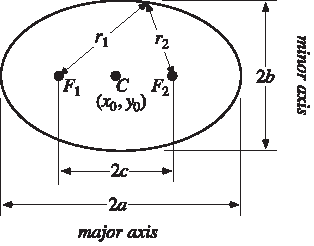
\includegraphics[width=\textwidth]{../Figures/ellipse/EllipseBipolar_700.pdf}
    \caption{Ellipse}\label{fig:ellipse}
\end{marginfigure}
Where the value $a$ is commnly refered as \textit{semimajor axis}, the points $F_1$ and $F_2$ as \textit{foci} and the half point between the foci is refered as the \textit{origin} of the coordinate system.

\subsection{Derivation of the equation}

To derive the a;gebraic form of the ellipse from its definition, we start by translating the definition of the ellipse into an algebra representation.
First, we represent the foci as $F_1=(c,0)$ and $F_2=(-c,0)$.
Now, we recall the equation to compute the distance between two points, $d=\sqrt{(x_1-x_2)^2+(y_1-y_2)^2}$.
Since we want to find the points in the plane that satisfies the definiiton of the ellipse, we are going to find the distance between the foci and all the plane,
\begin{gather*}
    \sqrt{(x-c)^2+y^2} + \sqrt{(x+c)^2+y^2}.
\end{gather*}
Now we are going to apply the restricction that the sum of those distances are equal to $2a$,
\begin{gather*}
    \sqrt{(x-c)^2+y^2} + \sqrt{(x+c)^2+y^2} = 2a.
\end{gather*}

With this equation we are going to apply several algebraic tricks\footnote{
    Basically we are going to get rid of the radicals ($\sqrt{x}$) and fractions.
} to simplify the equation.
Let's start by isolating one distance and then squaring the equation,\marginnote{
    \begin{gather*}
        \qty[2a - \sqrt{(x+c)^2+y^2}]\qty[2a - \sqrt{(x+c)^2+y^2}] \\
        4a^2 -4a\sqrt{(x+c)^2+y^2} + (x+c)^2+y^2
    \end{gather*}
}
\begin{align*}
    \sqrt{(x-c)^2+y^2} &= 2a - \sqrt{(x+c)^2+y^2} \\
    \qty[\sqrt{(x-c)^2+y^2}]^2 &= \qty[2a - \sqrt{(x+c)^2+y^2}]^2 \\
    (x-c)^2+y^2 &= 4a^2 -4a\sqrt{(x+c)^2+y^2} + (x+c)^2+y^2 \\
    x^2-2cx+c^2+y^2 &= 4a^2 -4a\sqrt{(x+c)^2+y^2} + x^2 +2cx +c^2 +y^2\\
    \cancelto{0}{x^2}
    -2cx+c^2
    +\cancelto{0}{y^2} &= 4a^2 -4a\sqrt{(x+c)^2+y^2} + \cancelto{0}{x^2} +2cx +c^2 +\cancelto{0}{y^2}\\
    -4cx &= 4a^2 -4a\sqrt{(x+c)^2+y^2}.
\end{align*}

Now, we are going to solve for the distance $\sqrt{(x+c)^2+y^2}$,
\begin{align*}
    -4cx &= 4a^2 -4a\sqrt{(x+c)^2+y^2} \\
    4a\sqrt{(x+c)^2+y^2} &= 4a^2 + 4cx \\
    \sqrt{(x+c)^2+y^2} &= \frac{4a^2 + 4cx}{4a} \\
    \sqrt{(x+c)^2+y^2} &= a + \frac{cx}{a}.
\end{align*}

Now we square it again\footnote{
    \begin{gather*}
        (x+c)^2 = x^2 +2cx + c^2
    \end{gather*}
},
\begin{align*}
    \qty[\sqrt{(x+c)^2+y^2}]^2 &= \qty[a + \frac{cx}{a}]^2 \\
    x^2 +\cancelto{0}{2cx} + c^2 + y^2 &= a^2 +\cancelto{0}{2cx} + \frac{c^2x^2}{a^2} \\
    x^2 + c^2 + y^2 &= a^2 + \frac{c^2x^2}{a^2}.
\end{align*}

Now we multiply the equation by $a^2$ to transform the fraction term into a non fraction term,
\begin{align*}
    \left[x^2 + c^2 + y^2\right. &= \left.a^2 + \frac{c^2x^2}{a^2}\right]a^2 \\
    a^2x^2 + a^2c^2 + a^2y^2 &= a^4 + c^2x^2 \\
    a^2x^2 - c^2x^2 + a^2y^2 &= a^4 - a^2c^2  \\
    x^2\qty(a^2 - c^2) + a^2y^2 &= a^2\qty(a^2 - c^2).
\end{align*}

We can simplify the expression by using the pythagorean relation $a^2 = b^2 + c^2,\to b^2 = a^2-c^2$,
\begin{align*}
    x^2\cancelto{b^2}{\qty(a^2 - c^2)} + a^2y^2 &= a^2\cancelto{b^2}{\qty(a^2 - c^2)} \\
    b^2x^2 + a^2y^2 &= a^2b^2.
\end{align*}

Finally, we divide all the expression by $a^2b^2$,
\begin{align*}
    \frac{x^2}{a^2} + \frac{y^2}{b^2} &= 1,
\end{align*}
where $b$ is normally known as the \textit{semiminor axis} and $a$ as \textit{semimajor axis}\footnote{
    This equation is similar to the \textit{unit} circle equation ($x^2 + y^2 = 1$), where $a=1$ and $b=1$.
}.

\subsection{General equation}

From the derivation we assume that the origin of the ellipse is at $(0,0)$, so now we are going to see how to modify the equation to shift that origin point to any other point inside the plane.
Using the same notation from the circle, we are going to shifts the ellipse to the coordinate $(h,k)$\footnote{Due to equating the function to $1$ the domain and range is $x\in\qty[h-a,h+a]$ and $f(x,y)\in\qty[k-b,k+b]$},
\begin{align*}
    \frac{\qty(x-h)^2}{a^2} + \frac{\qty(y-k)^2}{b^2} &= 1.
\end{align*}

\begin{note}{Expanded form}{~}
Now we are going to expand the expression,
\begin{align*}
    \frac{\qty(x-h)^2}{a^2} + \frac{\qty(y-k)^2}{b^2} &= 1 \\
    \frac{1}{a^2}\qty(x^2-2xh+h^2) + \frac{1}{b^2}\qty(y^2-2yk+k^2) &= 1 \\
    \frac{x^2}{a^2} + \frac{y^2}{b^2}
    -\frac{2xh}{a^2} -\frac{2yk}{b^2}
    +\frac{h^2}{a^2} + \frac{k^2}{b^2} &= 1
\end{align*}

As same with the circle equation, we can approch this as a two variable function $f(x,y)$ equated to $1$, $f(x,y)=1$.
However, we need to take into account that this is not a bijective function, which leads to have a bounded domain and range with no inverse function.
\end{note}

\subfile{exercise.tex}

\end{document}
